\documentclass[11pt]{article}
\usepackage{amsmath,amssymb}
\usepackage[margin=1in]{geometry}
\usepackage[T1]{fontenc}
\usepackage{newcent}
\usepackage{microtype}
\usepackage{graphicx}
\graphicspath{{figures/pdf/}{../figures/pdf/}}
\usepackage[font=small,labelfont=bf]{caption}
\usepackage[section]{placeins}
\usepackage{array}
\usepackage{titlesec}
\usepackage[hidelinks,pdfusetitle]{hyperref}

\renewcommand{\thesection}{\Roman{section}}
\counterwithout{subsection}{section}
\titleformat{\section}{\normalfont\Large\bfseries}{\thesection.}{.6em}{}
\titleformat{\subsection}{\normalfont\large\bfseries}{\thesubsection.}{.6em}{}
\titlespacing*{\paragraph}{0pt}{.6ex}{1em}

\renewcommand{\topfraction}{.9}
\setlength{\textfloatsep}{12pt plus 2pt minus 2pt}
\setlength{\intextsep}{12pt plus 2pt minus 2pt}
\AddToHook{env/itemize/begin}{\setlength{\itemsep}{3pt}\setlength{\parskip}{0pt}}

\renewcommand{\thetable}{\Alph{table}}
\newenvironment{plaintable}{\par\medskip\noindent\begin{minipage}{\linewidth}\captionsetup{type=table,skip=3pt}\small
  \renewcommand{\arraystretch}{1.05}\setlength{\tabcolsep}{5pt}}{\end{minipage}\par\medskip}
\newcolumntype{L}[1]{>{\raggedright\arraybackslash}p{\dimexpr#1\linewidth-\tabcolsep\relax}}

\title{Quantum State Spaces of Nonrigid\\ Molecules and Their Complexes}
\author{Isaac AshLind}
\date{}

\newcommand{\R}{\mathbb{R}}
\newcommand{\conf}{\mathcal{C}}
\newcommand{\hilb}{\mathcal{H}}
\newcommand{\spin}{\mathcal{H}_{\mathrm{spin}}}
\newcommand{\act}{\mathbin{\cdot}}
\newcommand{\stat}{\chi_{\mathrm{stat}}}
\newcommand{\X}{\mathbf{X}}
\newcommand{\Pmat}{\mathbf{P}}
\newcommand{\Rmat}{\mathbf{R}}
\newcommand{\Uop}{\mathsf{U}}

\begin{document}
\maketitle

\begin{center}
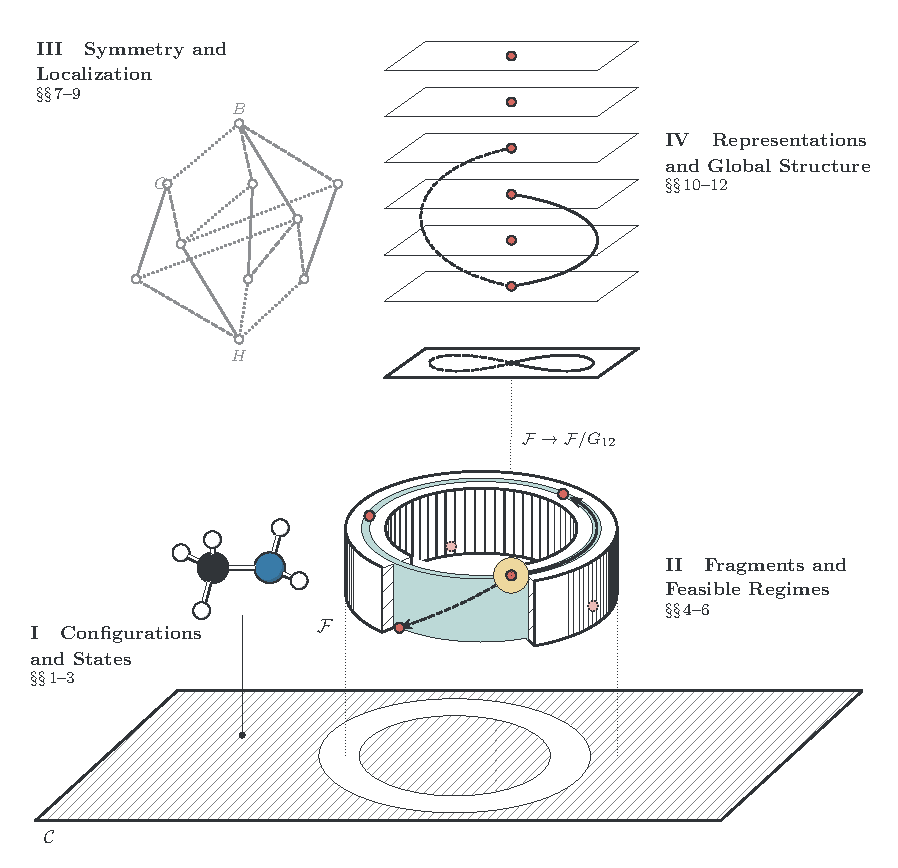
\includegraphics[width=\linewidth]{fig00-guide}
\end{center}
\clearpage

\section{Configurations and States}
\subsection{Configuration Space}
\label{sec:configuration}

Consider $N$ labeled nuclei in Euclidean space. 
Take
the \emph{configuration space} to be the set of all linear
maps $\X: \R^N \to\R^3$ that place the center of mass
at the origin.
In a Cartesian basis, represent $\X$ by a $3\times N$ matrix whose $i$th column $\mathbf
x_i=(x_i,y_i,z_i)^{\mathsf T}$ is the position of
nucleus $i$
\[
\X=
\begin{pmatrix}
    x_1 & x_2 & \cdots & x_N \\
    y_1 & y_2 & \cdots & y_N \\
    z_1 & z_2 & \cdots & z_N
\end{pmatrix}.
\]
The column vector $\mathbf m=(m_1,\ldots,m_N)^{\mathsf T}$
contains the nuclear masses. The centered configuration
space is
\[
\conf
=
\left\{
\X\in\hom(\R^N,\R^3):\X\mathbf m=0
\right\},
\qquad
\dim\conf=3N-3.
\]

The nuclei are sorted into types by their charge, mass,
and spin, with like nuclei permutable. We also allow global
inversion. For types indexed by $\alpha$, each having
multiplicity $n_\alpha$, the overall permutation and
inversion group\footnote{The complete nuclear
permutation--inversion (CNPI) group~\cite{BunkerEtAl1997}; see also
Longuet-Higgins~\cite{LonguetHiggins1963}.} is taken as
\[
S=\left(\prod_\alpha S_{n_\alpha}\right)
\times\{E,E^*\}.
\]

The inversion group $\{E,E^*\}$ is isomorphic to $C_2$.
We adopt the molecular literature's convention where
a star indicates inversion. Each element $s\in S$ is
therefore a permutation $\sigma$ or a
permutation--inversion $\sigma^*$.

As matrices, the $\X\in\conf$ form a vector space on which
permutations act by multiplication from the right
\[
s\act\X=\X\Pmat_s,
\qquad
\Pmat_{\sigma^*}=-\Pmat_\sigma.
\]
Here $\Pmat_\sigma$ reorders the columns according to
\[
\sigma\act(\mathbf x_1,\ldots, \mathbf x_N)
=
(\mathbf x_{\sigma^{-1}(1)},\ldots,\mathbf x_{\sigma^{-1}(N)}).
\]
With this convention, for $s,s'\in S$,
\[
s\act(s'\act\X)
=(\X\Pmat_{s'})\Pmat_s
=\X\Pmat_{s'}\Pmat_s
=(ss')\act\X.
\]
The matrices satisfy $\Pmat_{ss'}=\Pmat_{s'}\Pmat_s$. Multiplication by
these matrices on the right therefore defines a left
action of $S$ on $\conf$.

We can also act on $\X$ from the left with rotations
$r\in SO(3)$ via $3\times3$ rotation matrices $\Rmat(r)$
\[
r\act\X=\Rmat(r)\X.
\]
The actions commute by associativity
\[
r\act(s\act\X)=\Rmat(r)\X\Pmat_s=s\act(r\act\X).
\]
We drop the dots when the action is understood.

\begin{figure}[tb]
\centering
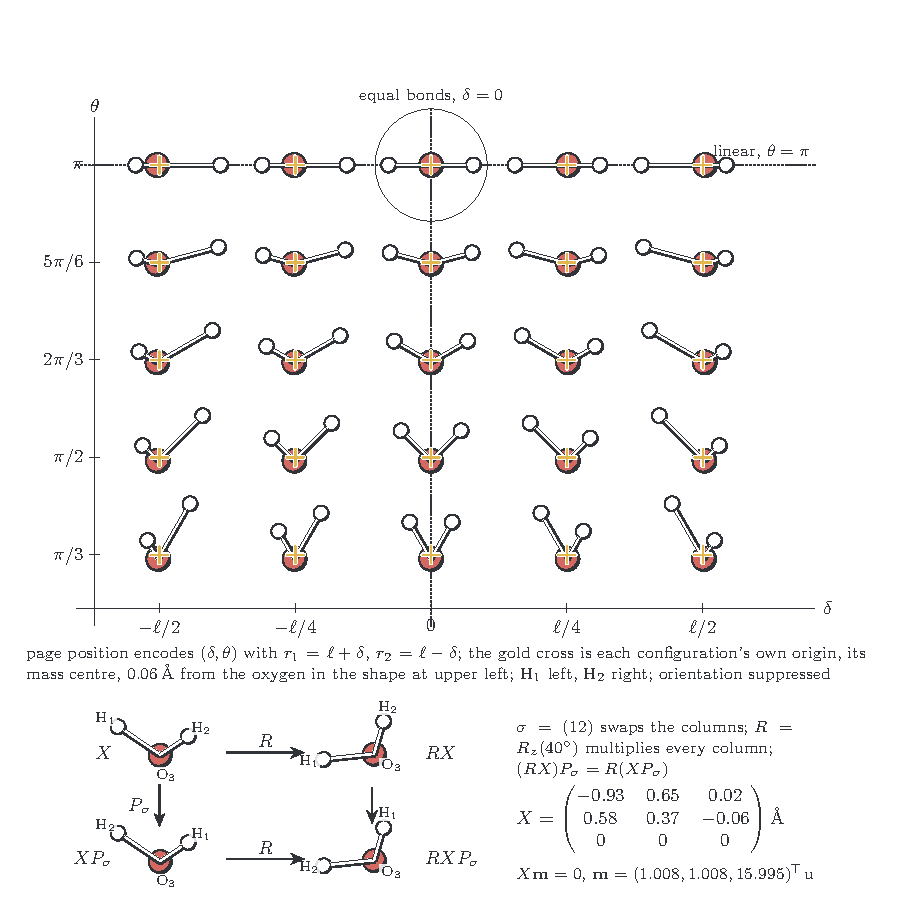
\includegraphics{fig01-configuration-space}
\caption{Configuration space. Each water shape sits at its bond asymmetry $\delta$ and bend angle
$\theta$. Symmetric shapes lie on the line $\delta=0$ and linear shapes on the line $\theta=\pi$. Below, a
rotation $\Rmat$ acts on the configuration matrix $\X$ from the left, and a permutation $\Pmat_\sigma$ and
the inversion $E^*$ act from the right.}
\label{fig:1}
\end{figure}

\subsection{Ambient Hilbert Space}
\label{sec:ambient}

The \emph{ambient Hilbert space} for our configuration space,
including the spin of the nuclei, is
\[
\hilb_{\mathrm{amb}}=L^2(\conf)\otimes\spin,
\qquad
\spin=\bigotimes_{i=1}^{N}\mathbb C^{2I_i+1}.
\]
Here $L^2(\conf)$ uses the translation-invariant volume
measure $d\X$ up to normalization.
The $i$th nucleus has spin number $I_i$, and its
spin vectors lie in $\mathbb C^{2I_i+1}$. A general vector
in $\spin$ is a linear combination of products
$\xi_1\otimes\cdots\otimes\xi_N$, with factors ordered
by nuclear label.

The group $S$ permutes like-nucleus spin factors in the
same order as the configuration columns, with inversion
acting trivially
\[
s\act(\xi_1\otimes\cdots\otimes\xi_N)
=
\xi_{\sigma^{-1}(1)}\otimes\cdots\otimes
\xi_{\sigma^{-1}(N)},
\]
where $\sigma$ is the permutation underlying $s$.
The action extends linearly to all spin vectors.

A wavefunction is a square-integrable map
\[
\Psi:\conf\to\spin,
\qquad
\|\Psi\|^2
=
\int_{\conf}\|\Psi(\X)\|_{\spin}^2\,d\X<\infty.
\]
For example, if $\xi,\zeta\in\spin$ are orthonormal and
$\Psi(\X)=f_\xi(\X)\xi+f_\zeta(\X)\zeta$, then
\[
\|\Psi(\X)\|_{\spin}^2=|f_\xi(\X)|^2+|f_\zeta(\X)|^2,
\qquad
\|\Psi\|^2
=
\int_{\conf}\bigl(|f_\xi(\X)|^2+|f_\zeta(\X)|^2\bigr)\,d\X.
\]

As in $L^2(\R^n)$, we identify wavefunctions whose
difference has zero norm
\[
\Psi\sim\Phi
\quad\Longleftrightarrow\quad
\int_{\conf}
\|\Psi(\X)-\Phi(\X)\|_{\spin}^2\,d\X=0.
\]

\begin{figure}[tb]
\centering
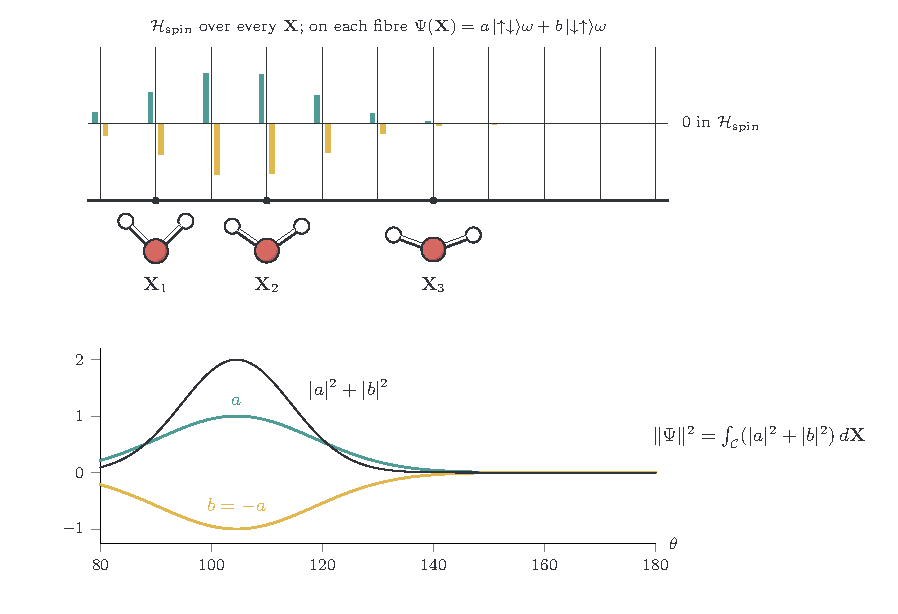
\includegraphics{fig02-ambient-hilbert-space}
\caption{Ambient Hilbert space. Over each configuration of a slice of $\conf$ stands a copy of the spin
space $\spin$. A state assigns to each configuration a vector with components $f_\xi$ and $f_\zeta$, and
$\|\Psi\|^2$ is the integral of $|f_\xi|^2+|f_\zeta|^2$ over $\conf$. The state drawn is unchanged by
rotations and antisymmetric under exchange, so $f_\zeta=-f_\xi$.}
\label{fig:2}
\end{figure}

\subsection{Physical Hilbert Space}
\label{sec:physical}

Exchange statistics select the \emph{physical Hilbert
space} $\hilb\subseteq\hilb_{\mathrm{amb}}$.

Inversion imposes no additional exchange-statistics
constraint, so we pass to $S/\langle E^*\rangle$,
identifying each coset $\{\sigma,\sigma^*\}$ with its
underlying permutation $\sigma$. Let $\sigma_\alpha$
be its restriction to nuclei of type $\alpha$, with
spin number $I_\alpha$. The statistics character is
\[
\stat(\sigma)
=
\prod_\alpha
\bigl(\operatorname{sgn}\sigma_\alpha\bigr)^{2I_\alpha}.
\]
Recall that $\Psi(\X)$ is a spin vector and $\sigma$ permutes
spin factors. Write
$(\Psi\circ\sigma)(\X)=\Psi(\sigma\X)$ and
$(\sigma\act\Psi)(\X)=\sigma\act\Psi(\X)$. Using the equivalence relation defined above,
the physical Hilbert space is
\[
\hilb
=
\left\{
\Psi\in\hilb_{\mathrm{amb}}
:
\Psi\circ\sigma
\sim
\stat(\sigma)\,\sigma\act\Psi,
\quad\forall\,\sigma\in S/\langle E^*\rangle
\right\}.
\]
In words, the physical wavefunctions are those which respect
exchange statistics under permutations in the configuration
space, with the spin factors reorganized accordingly.

The parity sectors of the physical Hilbert space are
\[
\hilb_\pm=\{\Psi\in\hilb:\Psi\circ E^*\sim\pm\Psi\},
\]
where $(\Psi\circ E^*)(\X)=\Psi(-\X)$.
They give the orthogonal decomposition
\[
\hilb=\hilb_+\oplus\hilb_-,
\qquad
\Psi=\Psi_++\Psi_-,
\qquad
\Psi_\pm(\X)=\frac12\bigl(\Psi(\X)\pm\Psi(-\X)\bigr).
\]
Extend $\stat$ to $S$ by ignoring the star, and define
the parity characters by
\[
\chi_\pm(\sigma)=1,
\qquad
\chi_\pm(\sigma^*)=\pm1.
\]
A physical wavefunction of parity $\pm$ then obeys
\[
\Psi_\pm\circ s
\sim
\stat(s)\chi_\pm(s)\,s\act\Psi_\pm,
\qquad\forall s\in S.
\]
Here composition acts on the configuration argument,
while $s\act\Psi_\pm$ acts on the spin factors.

\begin{figure}[tb]
\centering
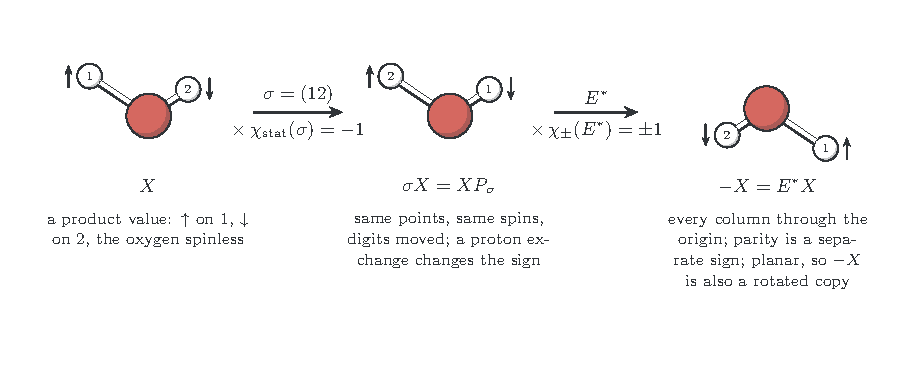
\includegraphics{fig03-physical-hilbert-space}
\caption{Physical Hilbert space. A relabeling $\sigma$ moves the digits and leaves each spin in its
place, so $\Psi(\sigma\X)=\stat(\sigma)\,\sigma\act\Psi(\X)$. The inversion $E^*$ sends every column
through the origin and multiplies $\Psi$ by the parity sign $\chi_\pm(E^*)=\pm1$.}
\label{fig:3}
\end{figure}

\section{Fragments and Feasible Regimes}
\subsection{Molecules, Fragments, and Complexes}
\label{sec:fragments}
\begin{itemize}
\item Partition the nuclei into fragments. One molecule is the
one-fragment case. Relative fragment positions and orientations remain in $\conf$.
\item For KRb + KRb, label potassium $1,2$ and rubidium $3,4$.
\end{itemize}
\[
\mathrm{KRb}+\mathrm{KRb}
\longrightarrow\mathrm K_2\mathrm{Rb}_2
\longrightarrow\mathrm K_2+\mathrm{Rb}_2,
\qquad S=\langle(12),(34),E^*\rangle\cong C_2^3.
\]
\[
G_{\mathrm{in}}=\langle(12)(34),E^*\rangle,
\qquad G_{\mathrm K}=\langle(12),E^*\rangle,
\qquad G_{\mathrm{Rb}}=\langle(34),E^*\rangle.
\]
\begin{itemize}
\item Each channel group has order $4$. Any two generate $S$.
Separate group inclusion from physical accessibility.
\item For $^{40}\mathrm K{}^{87}\mathrm{Rb}$, experiment finds
near-conservation of nuclear spin and corresponding product rotational
parities.\footnote{Hu et al.~\cite{HuEtAl2021}.}
Symmetry gives allowed sectors, not yields.
\item Choose a reference geometry to count versions.
\end{itemize}

\begin{figure}[tb]
\centering
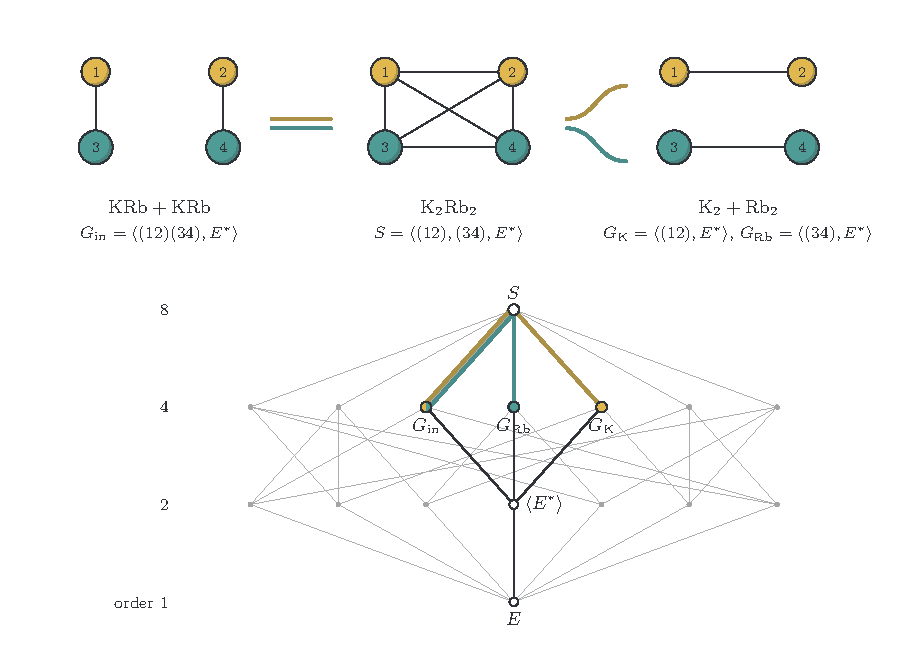
\includegraphics{fig04-molecules-fragments-complexes}
\caption{Molecules, fragments, complexes. The same four nuclei are grouped three ways along
$\mathrm{KRb}+\mathrm{KRb}\to\mathrm K_2\mathrm{Rb}_2\to\mathrm K_2+\mathrm{Rb}_2$, each grouping with its
permutation--inversion group. Gold follows the potassium nuclei and teal the rubidium nuclei. Below, the
same two strands run through the lattice of the sixteen subgroups of $S$.}
\label{fig:4}
\end{figure}

\subsection{Symmetry Groups and Versions}
\label{sec:groups-versions}

The construction so far accommodates all possible
arrangements of nuclei without imposing energetic or
experimental restrictions. Experimental resolution informs the choice of a feasible
regime with a group $G\leq S$ of feasible operations. For a given configuration $\X$,
there is a natural minimal symmetry $H$ consisting of the
permutation--inversions equivalent to rotations in $SO(3)$. By looking at the subgroup lattice for $H\leq
G\leq S$ along with a reference configuration and chosen paths,
we can carve out the shapes of feasible regimes and
their symmetries without first specifying a potential.
This is a kinematic model. Which
regimes are accessible in practice is left to experiment.

Choose a reference configuration $\X_0$ and look at its orbit
under rigid rotations,
\[
SO(3)\X_0=\{r\X_0:r\in SO(3)\}.
\]
Its point group is the subgroup
\[
H
=
\{h\in S:h\X_0\in SO(3)\X_0\}.
\]
The point group $H$ stabilizes the rotational orbit of $\X_0$.
Thus, for every $h\in H$, there is a rotation $\Rmat_h\in SO(3)$
such that
\[
h\X_0=\Rmat_h\X_0.
\]
For nonlinear $\X_0$, this rotation is unique. The rotational
orbit $SO(3)\X_0$ describes the rigid reference, and $G=H$ is
the minimal feasible regime.

A rearrangement is described by a continuous path
\[
\gamma:[0,1]\to\conf
\]
beginning at $\X_0$ and ending at a rotated,
permutation--inverted copy of $\X_0$,
\[
\gamma(0)=\X_0,
\qquad
\gamma(1)=rs\X_0,
\]
for some $r\in SO(3)$ and $s\in S$. The motion is
nonrigid if the path leaves $SO(3)\X_0$.

If the resolved motions correspond to
$s_1,\ldots,s_k\in S$, they generate the feasible group
\[
G=\langle H,s_1,\ldots,s_k\rangle,
\qquad
H\leq G\leq S.
\]
The cosets $G/H$ are the versions\footnote{The term
\emph{version} follows Bunker and Jensen~\cite{BunkerJensen1998}; the full set of versions is $S/H$,
while $G/H$ gives those accessible within the regime.}
accessible within the regime.

Adding an operation $s$ moves from $G$ to $\langle G,s\rangle$.

\begin{itemize}
\item Take CH$_3$NH$_2$ with five hydrogens of the same isotope.
Label methyl hydrogens $1,2,3$, amino hydrogens $4,5$, carbon $6$, and nitrogen $7$.
\item Choose the reference mirror plane through $1,6,7$, exchanging
$2$ with $3$ and $4$ with $5$.
\end{itemize}
\[
S=S_5\times\{E,E^*\},\qquad |S|=240,
\qquad H=\langle b\rangle,\qquad b=(23)(45)^*.
\]
\begin{itemize}
\item Keeping bonds restricts the candidates to the interval $[H,B]=\{G:H\leq G\leq B\}$ of the subgroup
lattice, where $B$ is the bond-preserving subgroup below.
Here $S_A$ permutes the labels in $A$.
\end{itemize}
\[
B=(S_{\{1,2,3\}}\times S_{\{4,5\}})\times\{E,E^*\},
\qquad |B|=24,
\qquad t=(123),\quad u=(45).
\]
\[
G_6=\langle H,t\rangle,\qquad |G_6/H|=3,
\qquad G_{12}=\langle H,t,u\rangle,\qquad |G_{12}/H|=6.
\]
\begin{itemize}
\item Above $G_6$, adding $u$, $E^*$, or $u^*$ gives three order-$12$
candidates. Any two extensions generate $B$.
\item Microwave and far-infrared spectra resolve torsion and inversion
in the $G_{12}$ regime.\footnote{Ilyushin et al.~\cite{IlyushinEtAl2005} and
Kr\k{e}glewski~\cite{Kreglewski2009}.}
The amino inversion includes a corrective $\pi/3$ methyl turn,
represented by $tu$.\footnote{Kleiner and Hougen~\cite{KleinerHougen2015}.}
\item Comparing the candidates through their species and spin weights is
the intended test; Sections~\ref{sec:species} and~\ref{sec:weights} carry
it out for $G_6$.
The full interval $[H,S]$ has $36$ subgroups, and $[H,B]$ has $10$.
\end{itemize}

\begin{figure}[p]
\centering
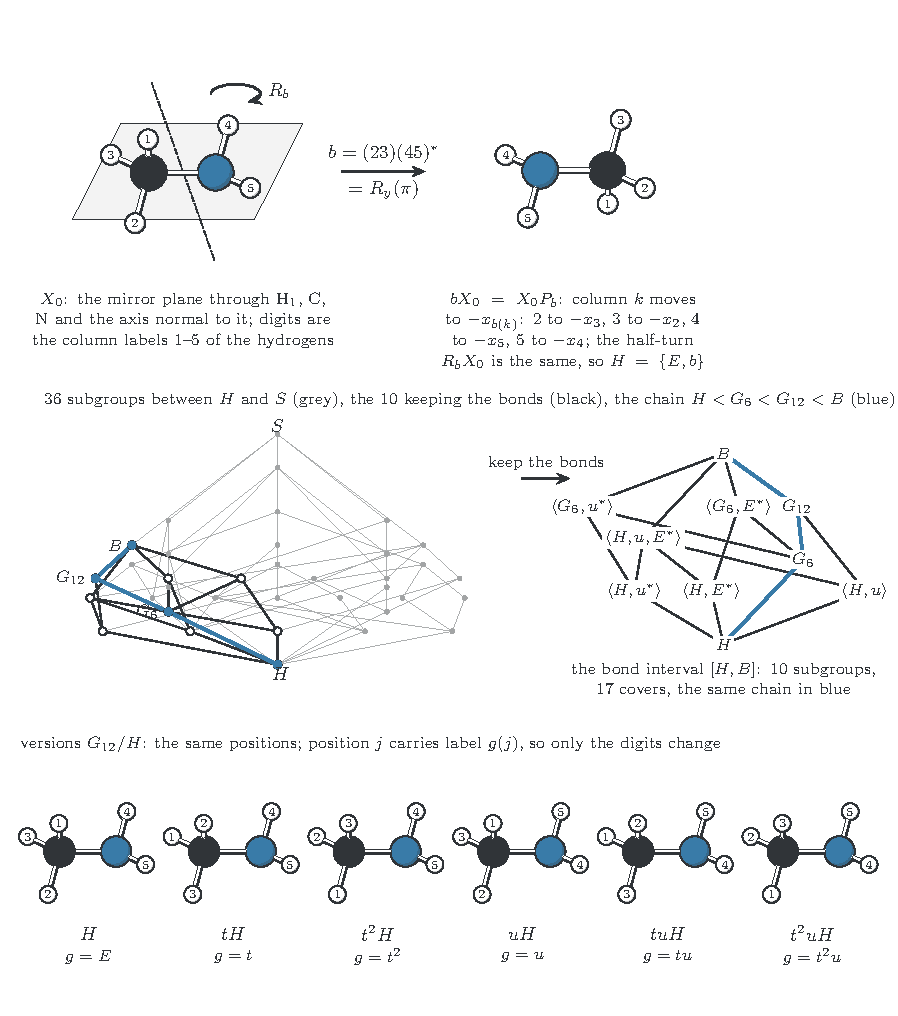
\includegraphics[width=\linewidth]{fig05-symmetry-groups-versions}
\caption{Symmetry groups and versions. At the top are methylamine's two fragments and the reference
$\X_0$, for which $b\X_0=\X_0\Pmat_b=\Rmat_b\X_0$. In the middle, the $10$ subgroups of $[H,B]$, which keep
the bonds, stand out from the $36$ of $[H,S]$. Each cover adds one generator, solid for $t$,
dashed for $u$, and dotted for a starred one. At the bottom are the six versions $G_{12}/H$.}
\label{fig:5}
\end{figure}

\subsection{Feasible Configuration Space}
\label{sec:feasible-space}
\begin{itemize}
\item Sweep chosen rearrangement paths through rotations and $G$.
Thicken in the normal directions to obtain a connected region
$\mathcal F\subseteq\conf$.
\item Require $s\mathcal F=\mathcal F$ for $s\in G$ and
$s\mathcal F\cap\mathcal F=\varnothing$ otherwise.
The copies are indexed by $S/G$, with $|G/H|$ reference versions in each.
\item Separation can be derived rather than assumed. Take $\mathcal F$ to be the connected component
through $\X_0$ of the union of all $S$-images of the thickened sweep. Every $s\in S$ permutes the
components, so $s\mathcal F$ either equals $\mathcal F$ or misses it. The stabilizer of $\mathcal F$
contains $G$ and equals $G$ unless the thickening is wide enough to merge copies.
\end{itemize}
\begin{figure}[tb]
\centering
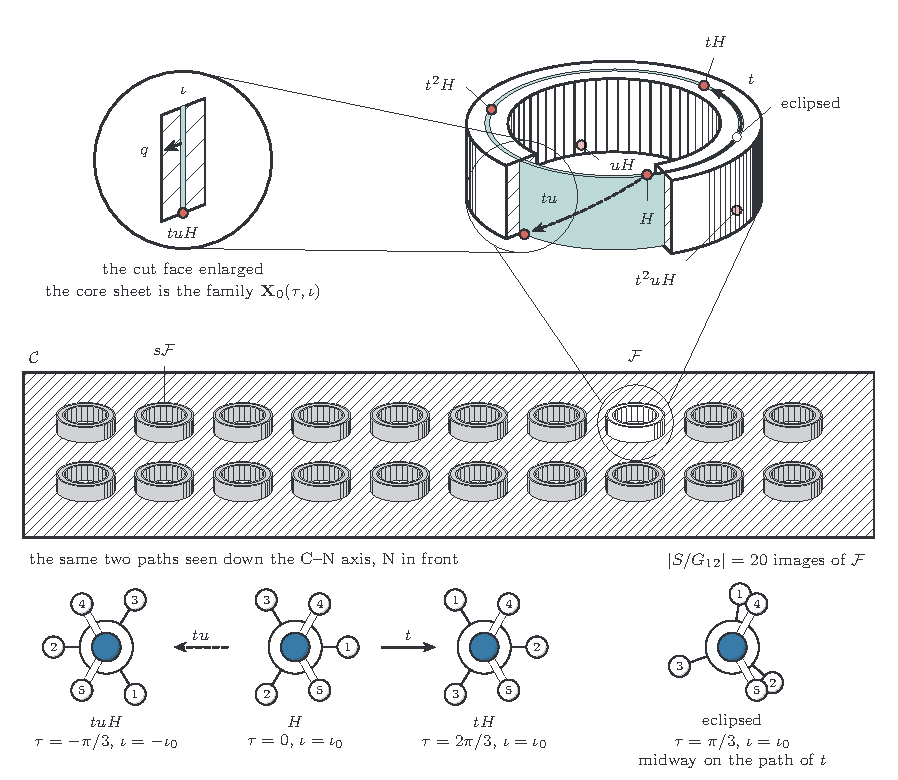
\includegraphics{fig06-feasible-configuration-space}
\caption{Feasible configuration space. The feasible region $\mathcal F$ has twenty images in $\conf$,
one for each coset in $S/G_{12}$. At the top, $\mathcal F$ is cut open as a solid. Its core sheet is the
family $\X_0(\tau,\iota)$, its thickness is the vibrations, and its cut face is enlarged at the left. At the
bottom, the two steps $t$ and $tu$ are seen down the C--N axis, with the eclipsed shape halfway along the
path of $t$.}
\label{fig:6}
\end{figure}
\[
S/H\longrightarrow S/G,\qquad sH\longmapsto sG.
\]
\begin{itemize}
\item For methylamine's $G_{12}$ regime, sweep the torsion angle $\tau$ around its circle
and the umbrella coordinate $\iota$ between the versions' values $\pm\iota_0$. Picture a short tube
$S^1\times[-\iota_0,\iota_0]$ of reference shapes $\X_0(\tau,\iota)$, thickened by the normal coordinates $q$,
with orientations over each shape.
\item The illustrated model assumes the product structure, connectedness,
and separation. The rigid specialization is recovered by freezing internal
shape and excluding rearrangements; see \hyperref[sec:example]{the example that closes the paper}.
\end{itemize}
\begin{itemize}
\item For an exact support restriction, use the whole symmetry-related union.
\end{itemize}
\[
\hilb_{\mathcal F}
=\left\{\Psi\in\hilb:
\Psi=0\text{ a.e. outside }\bigcup_{s\in S}s\mathcal F\right\}.
\]
\begin{itemize}
\item For open regions, compactly supported smooth packets, combined
with spin and projected onto exchange statistics, span this space densely.
Gaussians retain tails.
\item Tails can be measured without a potential. Every element of $S$ maps the union
$\bigcup_{s\in S}s\mathcal F$ to itself, so multiplying by its indicator function commutes with the
symmetry action and keeps the physical-state condition. A physical $\Psi$ splits into its parts inside and
outside the union, both physical. The norm of the outside part is the distance from $\Psi$ to
$\hilb_{\mathcal F}$.
\item Nested regions give nested state spaces. Group inclusion alone
does not specify geometric inclusion.
\end{itemize}

\section{Symmetry and Localization}
\subsection{Symmetry Species}
\label{sec:species}
\begin{itemize}
\item The irreducible representations of $G$ are its \emph{species}.
Pair spatial species with nuclear spin and compute spin weights.
\item Project a spatial state onto each species. Write
$\chi_\Gamma=\operatorname{tr}\Gamma$ and $d_\Gamma=\dim\Gamma$.
The projector retains all copies of that species.
\end{itemize}
\[
(\Uop_gf)(\X)=f(g^{-1}\X),\qquad
\mathsf P_\Gamma=\frac{d_\Gamma}{|G|}
\sum_{g\in G}\chi_\Gamma(g^{-1})\,\Uop_g.
\]
\[
w_\Gamma(f)=\frac{\|\mathsf P_\Gamma f\|^2}{\|f\|^2},
\qquad \sum_\Gamma w_\Gamma(f)=1,\qquad f\ne0.
\]
\begin{itemize}
\item Choose states at one version, specify their $H$ action, and induce
over $G/H$.\footnote{Harter~\cite{Harter1993}.} Start with a local vibrational ground state at fixed
rotational angular momentum.
\item One scalar state fixed by $H$ gives methylamine's three torsional
version states.
\end{itemize}
\[
\mathbb C[G_6/H]\cong\mathrm A_1\oplus\mathrm E.
\]
\begin{itemize}
\item A less symmetric base point has a smaller point group and a larger induced space. With a trivial
point group, $\mathbb C[G_6]\cong\mathbb C[G_6/H]\oplus\mathrm A_2\oplus\mathrm E$. The added
$\mathrm A_2\oplus\mathrm E$ is induced from the sign of $H$, so it describes local states odd under $b$.
\item Follow species across subgroup inclusions.
\item Use double cosets to organize connections between versions.
\item For complexes, induce incoming channel states and restrict to
product groups.
\end{itemize}

\begin{figure}[tb]
\centering
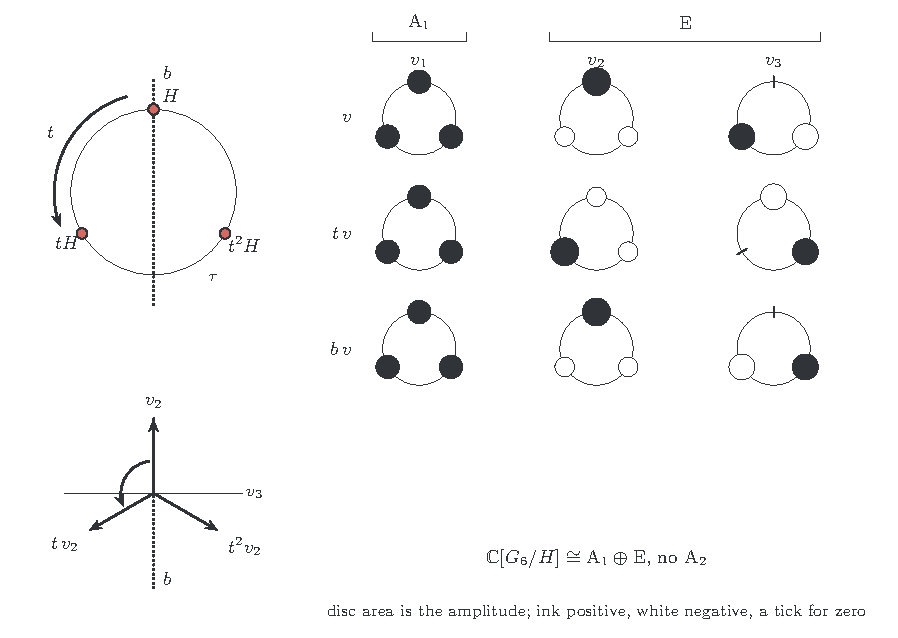
\includegraphics{fig07-symmetry-species}
\caption{Symmetry species. The three version sites sit on the torsion circle. The modes $v_1$, $v_2$,
$v_3$ are drawn with their images under $t$ and $b$, with a disc's area for the amplitude, ink for
positive, and white for negative. The functions on the sites split as
$\mathbb C[G_6/H]\cong\mathrm A_1\oplus\mathrm E$.}
\label{fig:7}
\end{figure}

\subsection{Nuclear Spin Weights}
\label{sec:weights}
\begin{itemize}
\item Restrict the nuclear-spin action of $S$ to the feasible group $G$.
Inversion acts trivially on spin, so only the permutation part of $G$ acts.
\item Decompose $\spin$ under $G$ into species, counting copies rather
than dimensions. For methylamine $\spin=(\mathbb C^2)^{\otimes5}\otimes\mathbb C^1\otimes\mathbb C^3$:
the five protons,
carbon-12, and nitrogen-14. Carbon and nitrogen are not permuted, so their factor carries $\mathrm A_1$ and
triples every count. Under $G_6$,
\end{itemize}
\[
(\mathbb C^2)^{\otimes5}\cong 12\,\mathrm A_1\oplus 4\,\mathrm A_2\oplus 8\,\mathrm E,
\qquad
\spin\cong 36\,\mathrm A_1\oplus 12\,\mathrm A_2\oplus 24\,\mathrm E,
\]
\begin{itemize}
\item so the eight copies of $\mathrm E$ fill sixteen of the protons' thirty-two
dimensions.
\item A spatial state of species $\Gamma$ and parity $\pm$ pairs with the
spin species $\Gamma'$ for which $\Gamma\otimes\Gamma'$ contains the
character $\stat\chi_\pm$ of the physical-state condition. On $G_6$,
$\stat=1$: even parity pairs each species with itself; odd parity exchanges
$\mathrm A_1$ with $\mathrm A_2$ and keeps $\mathrm E$.
\item The weight of a spatial level is the number of physical states it
carries, one for each copy of its partner species (Figure~\ref{fig:8}):
\end{itemize}
\begin{plaintable}
\caption{The physical weights of methylamine's spatial levels by parity.}
\label{tab:weights}
\centering
\begin{tabular}{@{}lrr@{}}
\hline
$\Gamma$ & even & odd\\
\hline
$\mathrm A_1$ & $36$ & $12$\\
$\mathrm A_2$ & $12$ & $36$\\
$\mathrm E$ & $24$ & $24$\\
\hline
\end{tabular}
\end{plaintable}

\begin{figure}[tb]
\centering
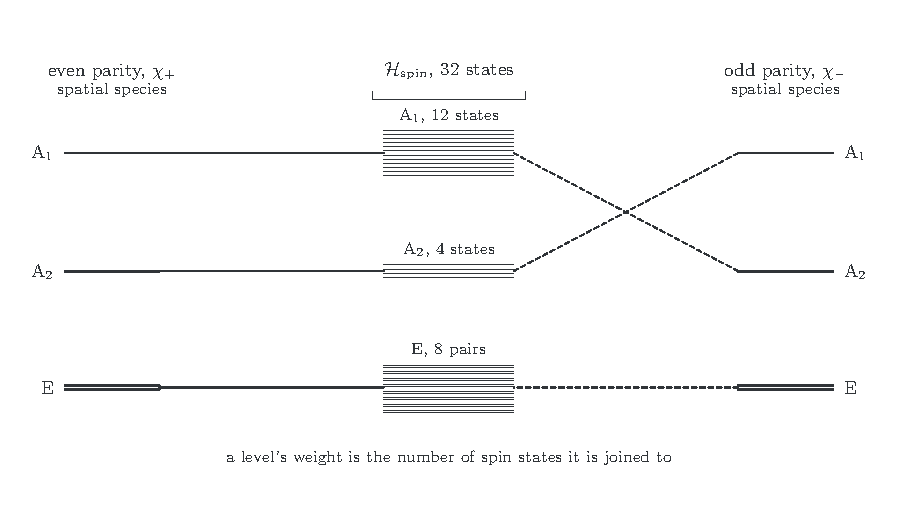
\includegraphics{fig08-nuclear-spin-weights}
\caption{Nuclear spin weights. The proton spin states split under $G_6$ as
$(\mathbb C^2)^{\otimes5}\cong12\,\mathrm A_1\oplus4\,\mathrm A_2\oplus8\,\mathrm E$, one line per state.
An even-parity spatial level joins the spin species of its own name. At odd parity $\mathrm A_1$ and
$\mathrm A_2$ trade partners and $\mathrm E$ keeps its own. A level's weight is the number of lines it
joins, times three for the spin states of nitrogen-14.}
\label{fig:8}
\end{figure}

\subsection{Localized States}
\label{sec:localized}
\begin{figure}[tb]
\centering
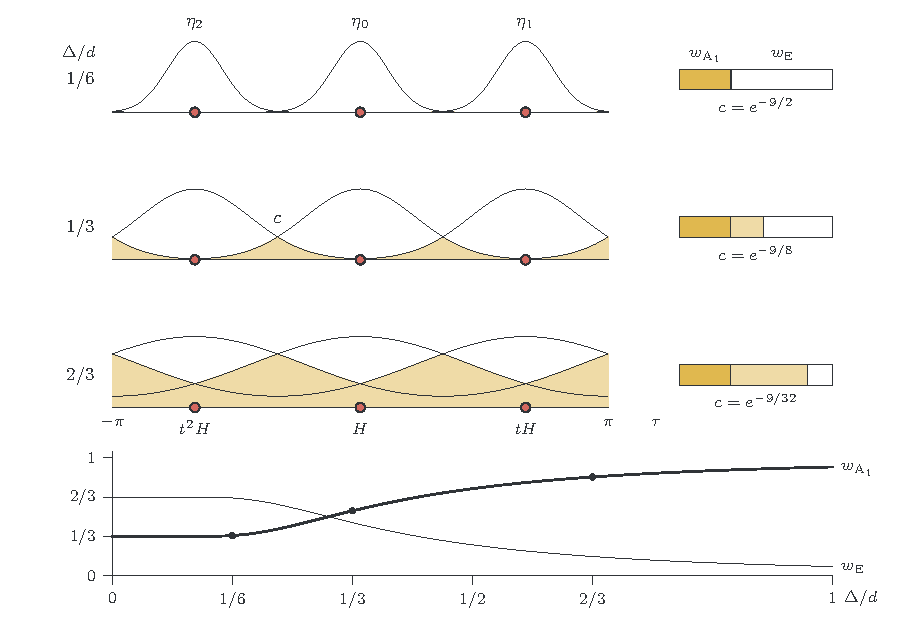
\includegraphics{fig09-localized-states}
\caption{Localized states. Three packets of width $\Delta$ sit on the unrolled torsion circle, a distance
$d$ apart, for $\Delta/d=1/6$, $1/3$, and $2/3$. The profiles are their densities, and neighbors cross at $c$
times the peak height. Each bar splits $w_{\mathrm A_1}=1/3+2c/3$ into the third a packet has with no
overlap, in gold, and the overlap part $2c/3$, in pale gold like the overlap regions. The rest of
the bar
is $w_{\mathrm E}=2(1-c)/3$. The rows have $c=e^{-9/2}$, $e^{-9/8}$, and $e^{-9/32}$, so in the top row the
overlap is nonzero but thinner than the line. Below, both shares are drawn against $\Delta/d$ with the three
rows marked. The packets are illustrative, and their overlap is that of planar Gaussians.}
\label{fig:9}
\end{figure}
\begin{itemize}
\item In $G_6$, choose a normalized real scalar packet $\eta_0$, fixed
by $H$ and localized near the reference rotational orbit.
Its translates sit at $H,tH,t^2H$.
\end{itemize}
\[
\eta_j(\X)=\eta_0(t^{-j}\X),\qquad j=0,1,2.
\]
\begin{itemize}
\item All pairwise overlaps equal $c=\langle\eta_0,\eta_1\rangle$.
The squared spatial projection shares of $\eta_0$ are
\end{itemize}
\[
w_{\mathrm A_1}=\frac{1+2c}{3},\qquad
w_{\mathrm E}=\frac{2(1-c)}{3},\qquad w_{\mathrm A_2}=0.
\]
\begin{itemize}
\item Independent packets span $\mathrm A_1\oplus\mathrm E$.
For a planar illustration, take equal Gaussians of position variance
$\Delta^2$ on an equilateral triangle of side $d$.
\end{itemize}
\[
c=\exp\!\left(-\frac{d^2}{8\Delta^2}\right).
\]
\begin{itemize}
\item With no overlap a packet is still one third $\mathrm A_1$, because
$\mathsf P_{\mathrm A_1}\eta_0=(\eta_0+\eta_1+\eta_2)/3$ averages it over the three versions. Overlap
adds $2c/3$
to that third. Gaussians have $c>0$ at every width, so $w_{\mathrm A_1}>1/3$.
\item A packet not fixed by $H$ splits as $\eta_0=\eta_0^++\eta_0^-$ with
$\eta_0^\pm=(\eta_0\pm\Uop_b\eta_0)/2$. Each projector commutes with $\Uop_b$, so the two parts
contribute to the shares separately. The even part follows the formulas above with its own overlap. The odd
part adds only $\mathrm A_2$ and $\mathrm E$, with total weight
$\|\eta_0^-\|^2=(1-\langle\eta_0,\Uop_b\eta_0\rangle)/2$, which vanishes as $\eta_0$ becomes fixed by $H$.
\item Overlaps $\langle\eta_0,\Uop_s\eta_0\rangle$ with $s\notin G$ measure how far a packet leaks into
the other copies of $\mathcal F$. Where they vanish, the shares under $S$ follow from those under $G$
through the branching of species. Otherwise they enter the shares as $c$ does.
\item Add $u$-related packets for the six versions in $G_{12}/H$.
Resolve the $u$ action through sums and differences.
\item Pair with spin and impose the feasible support restriction
of Section~\ref{sec:feasible-space}, when required.
\item Treat symmetry-enforced nodes with the required pointwise regularity.
\end{itemize}

\section{Representations and Global Structure}
\subsection{Position Representation}
\label{sec:position}
\begin{itemize}
\item Choose a body frame and a mass-orthonormal normal frame $\mathbf e_\alpha(a)$.
Use $r$ for orientation, $a$ for internal shape, and $q$ for normal coordinates.\footnote{For one
large-amplitude coordinate this is the nonrigid bender of Hougen, Bunker, and Johns~\cite{HougenBunkerJohns1970}.}
\end{itemize}
\[
\varphi(r,a,q)=\Rmat(r)\left(\X_0(a)+\sum_{\alpha=1}^{n_q}q_\alpha\mathbf e_\alpha(a)\right),
\qquad\psi(r,a,q)=\Psi\bigl(\varphi(r,a,q)\bigr).
\]
\begin{itemize}
\item On a regular chart $\varphi:\mathcal U\to\conf$, pull back the configuration measure.
Here $dr$ is normalized Haar measure and $j_\varphi$ is the chart density.
\end{itemize}
\[
d\mu=j_\varphi(a,q)\,dr\,da\,dq,
\qquad
\|\Psi\|_{\varphi(\mathcal U)}^2
=\int_{\mathcal U}\|\psi(r,a,q)\|_{\spin}^2\,d\mu.
\]
\begin{itemize}
\item The generalized states $|r,a,q\rangle$ resolve the chart identity with $d\mu$.
\item A state is a function on $\conf$ and needs no frame. A frame enters only when a state is written in a
chart, and changing the frame is a gauge transformation. Motions that carry no angular momentum define a
connection on $\mathcal F$ whose curvature couples rotation to shape, and no choice of frame removes
it.\footnote{Littlejohn and Reinsch~\cite{LittlejohnReinsch1997}.}
\item The feasible region avoids collinear and coincident shapes, so rotations act on it freely. Charts glued
by the transition maps below then cover it without a global body frame.
\item Write $x=(r,a,q)$. Carry each configuration action through the
source and target charts. For $s\in S$, solve for $x'=T_sx$.
\end{itemize}
\[
T_s=\varphi_{\mathrm{target}}^{-1}\circ s\circ\varphi_{\mathrm{source}}.
\]
\begin{itemize}
\item On a symmetry-invariant reference family, first find the new
shape $a'$ and compensating rotation $\mathbf A_s(a)$. Expand the transformed
normal frame in the target frame to obtain $\mathbf M_s(a)$.
\end{itemize}
\[
\begin{aligned}
\X_0(a)\Pmat_s&=\mathbf A_s(a)\X_0(a'),\\
\mathbf e_\alpha(a)\Pmat_s&=\mathbf A_s(a)\sum_\beta\mathbf e_\beta(a')\,[\mathbf M_s(a)]_{\beta\alpha},\\
T_s(r,a,q)&=\bigl(r\mathbf A_s(a),a',\mathbf M_s(a)q\bigr).
\end{aligned}
\]
\begin{itemize}
\item Here $\mathbf A_s(a)$ is the matrix of a rotation, and $r\mathbf A_s(a)$
denotes the orientation whose matrix is $\Rmat(r)\mathbf A_s(a)$; the same
reading applies to $r\Rmat_z(\omega)$ below.
\item This is exact on the normal chart. Finding $a'$ uses the chosen
shape coordinates, and the normal-frame expansion is linear algebra.
\item The invariance is required of the family, not of one configuration. Rotations and $G$ preserve the
mass-weighted distance, in which the $\mathbf e_\alpha(a)$ are orthonormal, and map the rotated family
$\Rmat(r)\X_0(a)$ to itself. So the nearest-point map onto the family, defined near it, commutes with them.
A configuration displaced from $\X_0$ along normal directions alone maps back to $\X_0$. Its own point group
may be smaller than $H$, but the point group of its base point is $H$.
\item A lab rotation $r_0$ gives $T_{r_0}(r,a,q)=(r_0r,a,q)$.
The induced spatial operator is the inverse pullback. Permuting the
spin factors gives the physical-state condition.
\end{itemize}
\begin{figure}[tb]
\centering
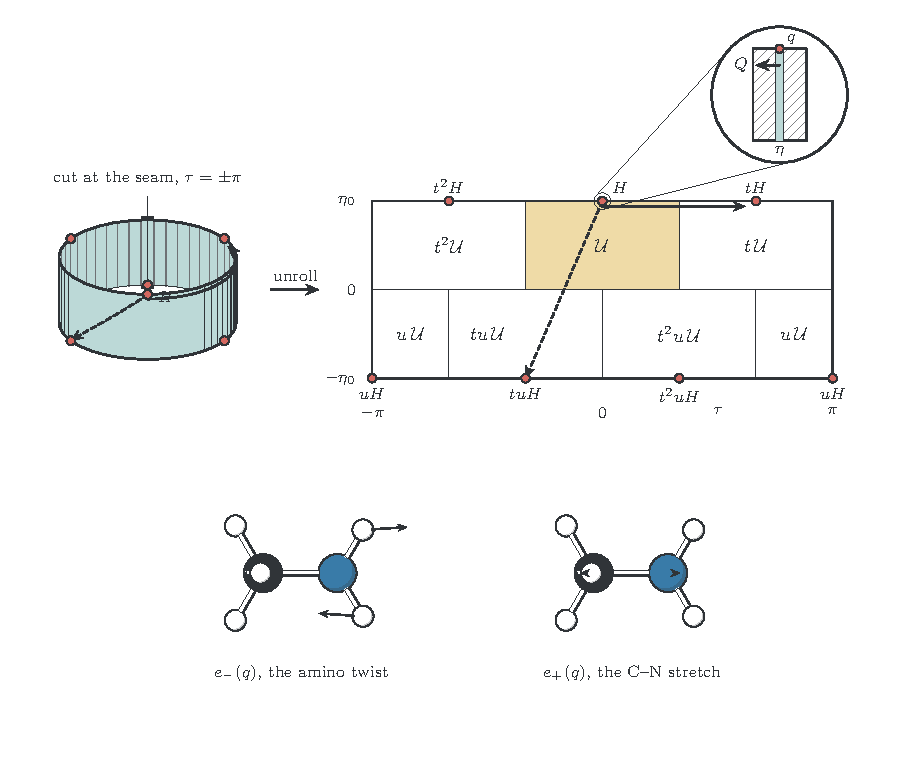
\includegraphics{fig10-position-representation}
\caption{Position representation. Without its vibrations the solid $\mathcal F$ is its core sheet,
which unrolls into the chart $[-\pi,\pi]\times[-\iota_0,\iota_0]$ with its six version cells. Over a point
$a$ of the chart, normal displacements $q$ and an orientation $r$ rebuild a configuration. The bottom row
shows the two normal directions at $a$.}
\label{fig:10}
\end{figure}
\[
(\Uop_s\psi)(x)=\psi(T_s^{-1}x),\qquad \Uop_s|x\rangle=|T_sx\rangle.
\]
\[
\psi(T_\sigma x)\sim\stat(\sigma)\,\sigma\act\psi(x).
\]
\begin{itemize}
\item With $\widetilde\psi=j_\varphi^{1/2}\psi$, the same operator in
the measure $dr\,da\,dq$ includes the density ratio.
\end{itemize}
\[
(\widetilde{\mathsf U}_s\widetilde\psi)(x)
=\left(\frac{j_\varphi(x)}{j_\varphi(T_s^{-1}x)}\right)^{1/2}
\widetilde\psi(T_s^{-1}x).
\]
\begin{itemize}
\item Use these formulas wherever the source and target charts apply.
Treat axial redundancy at linear configurations.
\end{itemize}

\begin{itemize}
\item For an explicit methylamine model, take the C--N axis as body $z$
and write the shape as $a=(\tau,\iota)$. In a periodic body frame,
$tu$ gives a half-turn of the frame, a $-\pi/3$ torsional shift,
and $\iota\mapsto-\iota$.\footnote{One reference family places the amino
hydrogens at $(\iota,\pm b_A,z_A)$ and the methyl hydrogens at angles
$\tau-2\pi(k-1)/3$, $k=1,2,3$, at fixed radius and height about
the C--N axis. Center the whole configuration as before.}
\item Twist the body frame by $\Rmat_z(-\rho\tau)$, with $\rho$ a chosen
frame parameter; we take $\rho=\frac12$, the analogue for one methyl top of
the symmetric internal-axis frame used for ethane by Mellor, Yurchenko, Mant,
and Jensen~\cite{MellorEtAl2019}. Retain two normal
coordinates $q_+,q_-$ chosen to transform evenly and oddly under $tu$.
These are symmetry-adapted coordinates, not vibrational eigenmodes.
\item The twist is a gauge choice. Physical results do not depend on $\rho$, but the form a Hamiltonian's
rotation--shape coupling takes in these coordinates does.
\end{itemize}
\[
\omega_{tu}=\pi-\frac{\rho\pi}{3},\qquad
x=(r,\tau,\iota,q_+,q_-),
\]
\[
T_{tu}x=\bigl(r\Rmat_z(\omega_{tu}),\tau-\pi/3,-\iota,q_+,-q_-\bigr),
\]
\[
(\Uop_{tu}\psi)(x)
=\psi\bigl(r\Rmat_z(-\omega_{tu}),\tau+\pi/3,-\iota,q_+,-q_-\bigr).
\]
\begin{itemize}
\item Six applications close through the seam of Section~\ref{sec:momentum}.
For proton exchange, $\stat(tu)=-1$.
\end{itemize}
\[
T_{tu}^{\,6}x
=\bigl(r\Rmat_z(-2\pi\rho),\tau-2\pi,\iota,q_+,q_-\bigr)\sim x,
\qquad \psi(T_{tu}x)\sim-(tu)\act\psi(x).
\]
\begin{itemize}
\item General normal coordinates replace the signs by matrices.
The rotational factor records the frame choice. It does not prescribe
dynamical rotational transport.
\item Versions and induced species depend on the base point only through the conjugacy class of its point
group. In $G_{12}$, a shape on one of the six lines $\tau\in(\pi/3)\mathbb Z$ is fixed by a conjugate of
$b$, so any reference there, the eclipsed shape included, gives the same versions and species up to
relabeling. A conjugate of $(23)^*$ fixes each of the six shapes $(\pi/6+k\pi/3,0)$,
$k=0,\ldots,5$, instead, and
no element but $E$ fixes any other shape. Which case describes the molecule is left to experiment.
\end{itemize}

\subsection{Covering Spaces and Monodromy}
\label{sec:covering}
\begin{figure}[tb]
\centering
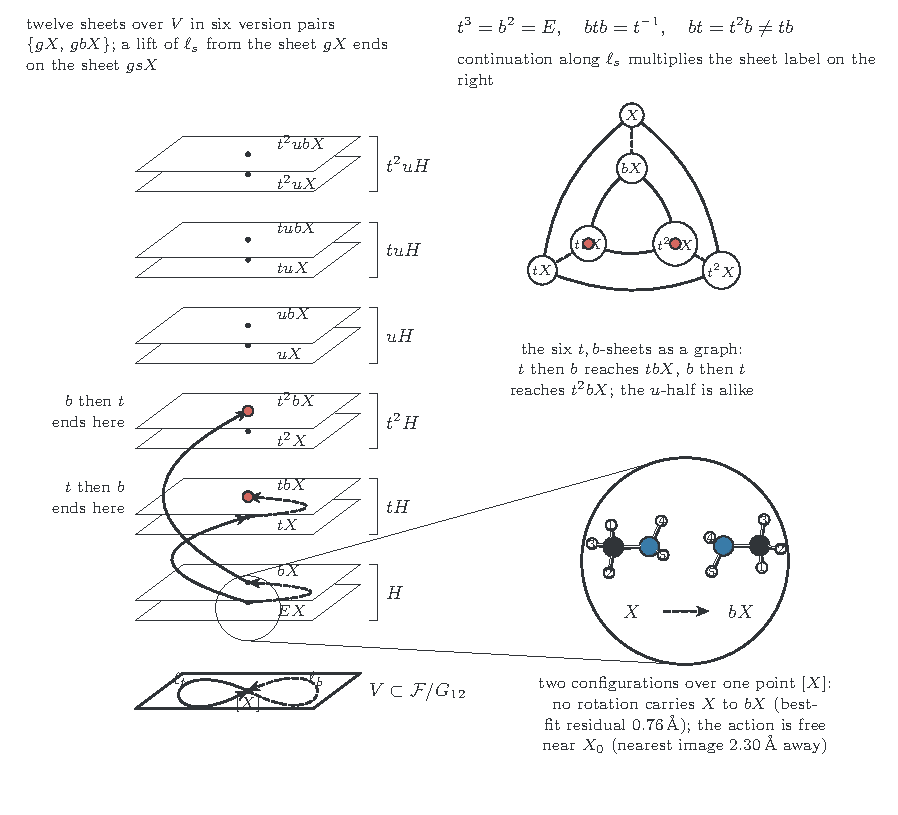
\includegraphics{fig11-covering-spaces-monodromy}
\caption{Covering spaces and monodromy. Over a patch of $\mathcal F/G$ stand the six sheets of the
$G_6$ block. In the base the paths $\gamma_t$ and $\gamma_b$ are loops. Lifted from $\X$ they end at $t\X$
and $b\X$. Taken in turn they end apart, $t$ then $b$ at $tb\X$ and $b$ then $t$ at $t^2b\X$. At the
right, the same sheets form a graph.}
\label{fig:11}
\end{figure}
\begin{itemize}
\item Versions label rotational orbits in $G/H$. Charts give local coordinates.
\item For methylamine, choose an $H$-invariant cell $\mathcal U$ whose
translates partition $\mathcal F$ up to their walls. Glue orientations,
normal coordinates, and wavefunctions across the walls.
\end{itemize}
\[
(G_{12}\times_H\mathcal U)/{\sim}\cong\mathcal F.
\]
\begin{itemize}
\item For a free action, $\mathcal F\to\mathcal F/G$ is a covering
with deck group $G$. A lifted chart transition induced by $g$
is a local expression of its deck transformation.
\item A rearrangement path $\gamma_s$ from $\X$ to $s\X$ projects to a loop in $\mathcal F/G$ through the
point $[\X]$,
the class of $\X$; the path is that loop's lift from $\X$. It stays in one
feasible component and records the sheet change, or
\emph{monodromy}.\footnote{Hatcher~\cite{Hatcher2002}, Section~1.3.}
\item Near a free reference configuration, twelve local sheets group
in pairs within six version cells. $G_{12}/H$ is a coset set, not a group.
\end{itemize}
\[
t^3=b^2=E,\qquad btb=t^{-1},\qquad bt=t^2b\ne tb.
\]
\begin{itemize}
\item A species sees $g$ through $\Gamma(g)$, with
$\Gamma(G)\cong G/\ker\Gamma$. On $G_6$, $\mathrm A_1$ sees no change,
while $\mathrm E$ retains noncommutativity.
\item Treat fixed configurations separately; the rigid orientation
construction is recovered in \hyperref[sec:example]{the example that closes the paper}.\footnote{Albert
et al.~\cite{AlbertEtAlOrientation}.}
\item Distinguish chart gluing from mechanical parallel
transport.\footnote{Littlejohn and Reinsch~\cite{LittlejohnReinsch1997}.}
A Berry interpretation needs
a specified state family and connection.
\end{itemize}

\subsection{Momentum Representation}
\label{sec:momentum}
\begin{itemize}
\item Expand the same states in rotational, internal, and normal modes,
subject to the chart identifications; the example below is a reduced
torsional model, not a transform of the full torsion--umbrella model.
\item For the product model $SO(3)\times S^1\times\R^{n_q}$, with $\iota$ held
at its reference value and omitted from the product (a reduced torsional
model), absorb the density into $\widetilde\psi=j_\varphi^{1/2}\psi$.
Use the measure $dr\,d\tau\,dq$, denoted by the subscript $0$.
\end{itemize}
\[
\langle r,\tau,q\mid JMK,m,p\rangle_0
=\frac{\sqrt{2J+1}\,D^J_{MK}(r)\,e^{im\tau}e^{ip\cdot q/\hbar}}
{\sqrt{2\pi}\,(2\pi\hbar)^{n_q/2}}.
\]
\[
J\in\mathbb N_0,\qquad -J\le M,K\le J,\qquad m\in\mathbb Z,
\qquad p\in\R^{n_q}.
\]
\begin{itemize}
\item The coefficients $\widehat\psi_{JMKm}(p)$ are spin vectors.
Sum over $J,M,K,m$ and integrate over $p$ for the inverse transform.
No energies are assigned; the product structure is assumed here.
\item Let the body frame close with a turn while the normal frame closes on itself.
\end{itemize}
\[
(r,\tau+2\pi,q)\sim\bigl(r\Rmat_z(-2\pi\rho),\tau,q\bigr),
\qquad D^J_{MK}(r\Rmat_z(\omega))=e^{-iK\omega}D^J_{MK}(r).
\]
\[
e^{2\pi i\kappa}=e^{2\pi i\rho K},\qquad
\kappa=m+\rho K=m+\frac12K,\qquad m\in\mathbb Z.
\]
\begin{itemize}
\item Periodic and twisted frames give integer and shifted labels for
the same states. Include normal-frame gluing when present.
\end{itemize}
\begin{itemize}
\item For periodic scalar torsion, take $f_m(\tau)=e^{im\tau}$,
with $T_t:\tau\mapsto\tau+2\pi/3$ and $T_b:\tau\mapsto-\tau$.
\end{itemize}
\[
\Uop_gf=f\circ T_g^{-1},\qquad
\Uop_tf_m=e^{-2\pi im/3}f_m,\qquad \Uop_bf_m=f_{-m}.
\]
\begin{itemize}
\item The species of the modes are those of Figure~\ref{fig:12}: $\mathrm A_1$
at $m=0$, an $\mathrm E$ pair when $3\nmid m$, and $\mathrm A_1\oplus\mathrm A_2$
(cosine, sine) at nonzero multiples of $3$; their spin partners follow the
rule of Section~\ref{sec:weights}. The coupled torsion and inversion of
methylamine lies outside the present example.
\end{itemize}

\begin{figure}[tb]
\centering
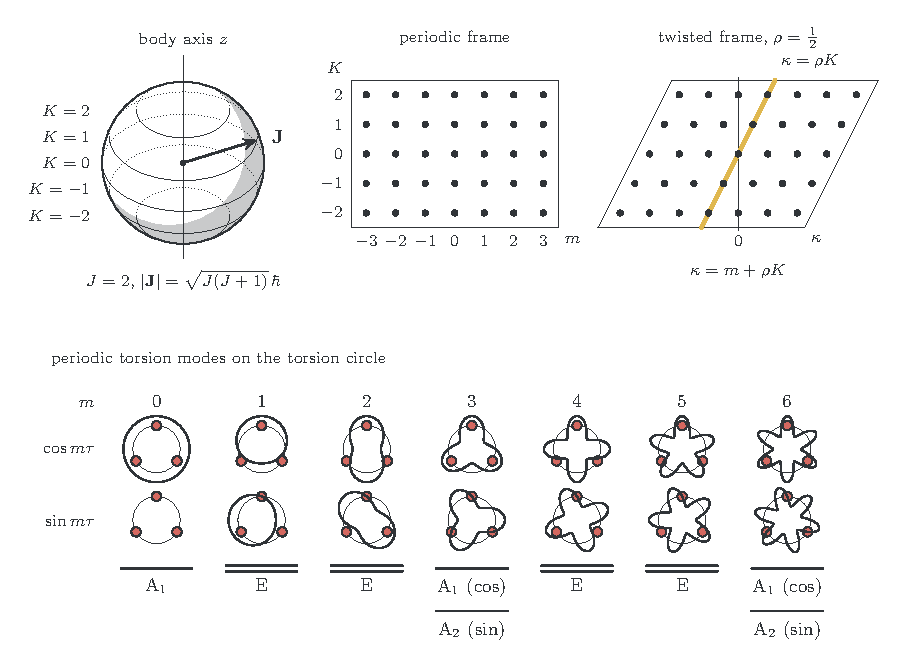
\includegraphics{fig12-momentum-representation}
\caption{Momentum representation. For $J=2$ the body-axis component $K$ takes five values on the
sphere $|\mathbf J|=\sqrt{J(J+1)}\,\hbar$, and the vector $\mathbf J$ drawn has $K=1$. The labels $(m,K)$
form a lattice in the periodic frame, and the twisted frame shears it to $\kappa=m+\frac12K$. The bottom
row shows the periodic torsion modes and their species under $G_6$. No energies are assigned.}
\label{fig:12}
\end{figure}

\clearpage
\section*{Example and Recovery of the Rigid Case}
\phantomsection\label{sec:example}
\pdfbookmark[1]{Example and Recovery of the Rigid Case}{example}
\begin{figure}[!ht]
\centering
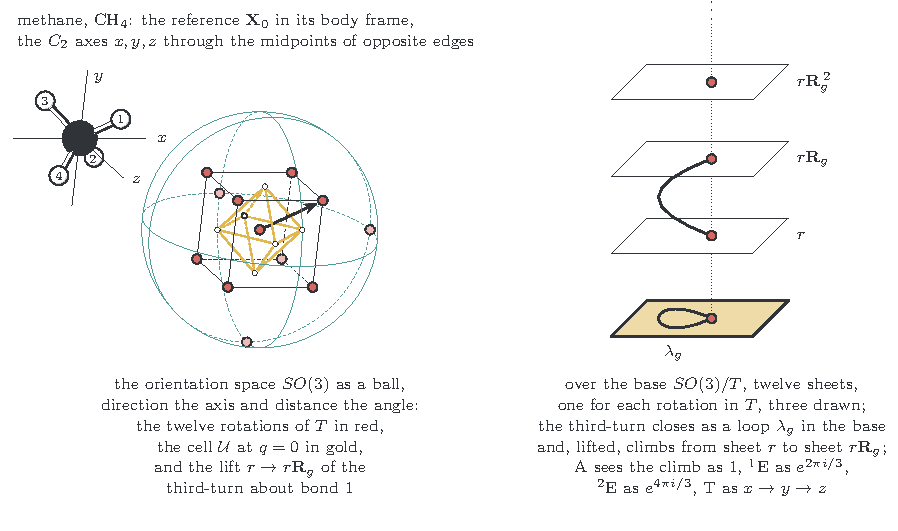
\includegraphics{fig13-rigid-orientation-ball}
\caption*{Rigid methane. On the left are the reference $\X_0$ in its body frame and the orientation
space $SO(3)$, drawn as a ball holding the twelve rotations of $T$. The arrow lifts the third-turn about
bond $1$. The gold cell is drawn as the octahedron dual to the cube of third-turns. This is exact in
Rodrigues coordinates, while in the ball the cell's edges bow outward. On the right is the covering, drawn
as in Figure~\ref{fig:11}.}
\end{figure}
We now run the construction of Sections~1 to~12 on one molecule, in order, and read off the
rigid case at the end. Take methane held at its tetrahedron, with protons $1$ to $4$ and carbon $5$. Each
step below carries the number of the section it applies. No energies are assigned.

\paragraph{\ref{sec:configuration}. Configuration Space}
Five nuclei with their center of mass fixed give the
twelve-dimensional space $\conf=\{\X\in\hom(\R^5,\R^3):\X\mathbf m=0\}$. The four protons are alike and
the carbon is unique, so $S=S_4\times S_1\times\{E,E^*\}$ has order $48$. In the body frame of the
figure, with $\ell=1.087$~\AA, the reference is
\[
\X_0=\frac{\ell}{\sqrt3}
\begin{pmatrix}
    1 & 1 & -1 & -1 & 0 \\
    1 & -1 & 1 & -1 & 0 \\
    1 & -1 & -1 & 1 & 0
\end{pmatrix}.
\]

\paragraph{\ref{sec:ambient}--\ref{sec:physical}. Ambient and Physical States}
Carbon-12 has spin zero, so
$\spin=(\mathbb C^2)^{\otimes4}\otimes\mathbb C^1$ is sixteen-dimensional. The protons are fermions, so
$\stat(\sigma)=\operatorname{sgn}\sigma$ and a physical state obeys
$\Psi\circ\sigma\sim\operatorname{sgn}\sigma\,\sigma\act\Psi$. It splits by parity into parts with
$\Psi_\pm(-\X)=\pm\Psi_\pm(\X)$.

\paragraph{\ref{sec:fragments}--\ref{sec:groups-versions}. Groups and Versions}
Methane is one molecule, so there are no fragments to
follow. Every relabeling carries the tetrahedron into its rotational orbit, the even ones as they stand
and the odd ones once starred (Table~\ref{tab:classes}). The point group of the reference is therefore
\[
H=\{h\in S:h\X_0\in SO(3)\X_0\}=T_d(\mathrm M)\cong S_4,
\qquad
h\X_0=\Rmat_h\X_0,
\qquad
\Rmat_{h_1h_2}=\Rmat_{h_2}\Rmat_{h_1}.
\]
The rotations $\Rmat_h$ form the cube group $O$, and those of the twelve unstarred $h$ form the
tetrahedral group $T$. Holding the tetrahedron admits no rearrangement, so the feasible group is $G=H$
and there is one version. The set $S/H$ has two elements. The second is the mirror-labeled tetrahedron
$E^*\X_0$, which no feasible motion reaches.

\paragraph{\ref{sec:feasible-space}. Feasible Configuration Space}
Thickening the orbit by its nine normal
coordinates gives $\mathcal F\cong SO(3)\times\R^9$. Each $h\in H$ maps $\mathcal F$ to itself, and
$E^*\mathcal F$ misses $\mathcal F$. So there are two copies, one for each coset in $S/G$, with one version
in each. The figure draws the factor $SO(3)$. The normal coordinates thicken it, and one may picture them
as a small disc about $q=0$.

\paragraph{\ref{sec:species}. Symmetry Species}
The species of $G$ are $\mathrm A_1$, $\mathrm A_2$,
$\mathrm E$, $\mathrm T_1$, and $\mathrm T_2$. Since $\mathbb C[G/H]\cong\mathrm A_1$, there are no version
modes. The structure lives instead in the orientation fiber and the normal coordinates of the one
version,
\[
\mathbb C[T]\cong\mathrm A\oplus{}^1\mathrm E\oplus{}^2\mathrm E\oplus3\,\mathrm T,
\qquad
T_{\X_0}\conf
\cong
\underbrace{\mathrm T_1}_{\text{along the orbit}}
\oplus
\underbrace{\mathrm A_1\oplus\mathrm E\oplus2\,\mathrm T_2}_{\text{the nine vibrations}}.
\]
The first is the space of functions on the twelve dots of the figure. The second is $\chi_{3N}$ of
Table~\ref{tab:classes}
less the translations $\mathrm T_2$ and the rotations $\mathrm T_1$.

\paragraph{\ref{sec:weights}. Nuclear Spin Weights}
From $\chi_{\mathrm{spin}}$ of Table~\ref{tab:classes},
$\spin\cong5\,\mathrm A_1\oplus\mathrm E\oplus3\,\mathrm T_2$, and $5+2+9=16$. A spatial species
$\Gamma$ of parity $\pm$ pairs with the spin species $\Gamma'$ for which $\Gamma\otimes\Gamma'$ contains
$\stat\chi_\pm$. That character is $\mathrm A_2$ at even parity and $\mathrm A_1$ at odd parity. One
physical state per copy gives the weights of Table~\ref{tab:isomers}.

\paragraph{\ref{sec:localized}. Localized States}
With $G=H$ there is no coset to induce over, so $H$ moves the
packet's orientation instead. Take a real packet $\eta_0(r,q)$ about the reference orientation and the
vibrational ground state. Its translates $\eta_h=\eta_0\circ T_h^{-1}$, for unstarred $h$, sit at the
twelve dots. If packets overlap by $c_3$ across a third-turn and by $c_2$ across a half-turn, the shares
of $\eta_0$ are
\[
w_{\mathrm A}=\frac{1+8c_3+3c_2}{12},\qquad
w_{{}^1\mathrm E}=w_{{}^2\mathrm E}=\frac{1-4c_3+3c_2}{12},\qquad
w_{\mathrm T}=\frac{3(1-c_2)}{4},
\]
which play the part of the shares in Section~\ref{sec:localized}. As a packet narrows against the spacing
of the
dots, $c_3$ and $c_2$ tend to zero and the shares to $d_\Gamma^2/12$. The twelve translates span $\mathbb
C[T]$.

\paragraph{\ref{sec:position}. Position Representation}
There is no shape coordinate, and the chart is
$\varphi(r,q)=\Rmat(r)\bigl(\X_0+\sum_{\alpha=1}^{9}q_\alpha\mathbf e_\alpha\bigr)$. In the chart, $h$ acts
through $\mathbf A_h=\Rmat_h$ and a fixed orthogonal $9\times9$ matrix $\mathbf M_h$, the matrix of
$\mathrm A_1\oplus\mathrm E\oplus2\,\mathrm T_2$,
\[
T_h(r,q)=(r\Rmat_h,\mathbf M_hq),\qquad
\psi(r\Rmat_h,\mathbf M_hq)\sim\stat(h)\chi_\pm(h)\,h\act\psi(r,q).
\]
The orientation chart is the ball of the figure. A point's direction is the axis of a rotation and its
distance from the center is the angle. The cell $\mathcal U$ holds the orientations nearer the center
than any other dot, together with all $q\in\R^9$. In Rodrigues coordinates $\tan(\omega/2)\,\mathbf n$,
for the turn by $\omega$ about the unit axis $\mathbf n$, its orientation part is the octahedron
$|x|+|y|+|z|\le1$. The six quarter-turns sit at its vertices and the third-turns at
$(\pm1,\pm1,\pm1)$, as the figure shows at $q=0$. The translates $T_h\mathcal U$ of unstarred $h$ tile
$\mathcal F$, so $(T\times\mathcal U)/{\sim}\cong\mathcal F$. Each face is the midplane to one third-turn
$\Rmat_g$ and is glued to the opposite face by $T_g^{-1}$, a third of a twist in orientation and
$\mathbf M_g^{-1}$ on the vibrations. With its faces glued, $\mathcal U$ becomes $\mathcal F/T$, the
bundle $SO(3)\times_T\R^9$ over $SO(3)/T$.

\paragraph{\ref{sec:covering}. Covering Spaces and Monodromy}
The map $\mathcal F\to\mathcal F/H$ is a covering
with deck group $H$ and twenty-four sheets. Its unstarred half $\mathcal F\to\mathcal F/T$ has twelve
sheets, the cells of the figure, and over $q=0$ it is the covering $SO(3)\to SO(3)/T$. The remaining factor
$O/T\cong C_2$, the starred half, is where parity enters. A third of a turn about the bond to
hydrogen~$1$ returns $\X_0$ with protons $2$, $3$, $4$ cycled. Its path $\gamma_g$ runs from $r$ to
$r\Rmat_g$, out of the central cell through a face and onto the next sheet, and in the quotient it is a
loop. A species $\Gamma$ sees this climb through $\Gamma(g)$. So $\mathrm A(g)=1$,
${}^1\mathrm E(g)=e^{2\pi i/3}$, ${}^2\mathrm E(g)=e^{4\pi i/3}$, and $\mathrm T(g)$ cycles the axes $x$,
$y$, $z$. The monodromy groups $T/\ker\Gamma$ are $1$, $C_3$, $C_3$, and $T$.

\paragraph{\ref{sec:momentum}. Momentum Representation}
On $SO(3)\times\R^9$ there is no torsional label, and
the momentum states are
\[
\langle r,q\mid JMK,p\rangle_0=\frac{\sqrt{2J+1}\,D^J_{MK}(r)\,e^{ip\cdot q/\hbar}}{(2\pi\hbar)^{9/2}},
\qquad
D^J_{MK}(r\Rmat_z(2\pi/3))=e^{-2\pi iK/3}D^J_{MK}(r),
\]
the second in the frame with $z$ along the bond to hydrogen~$1$. This is the seam rule of
Section~\ref{sec:momentum}
with $\omega=2\pi/3$. So $\Uop_g$ multiplies the ring $K$ by $e^{2\pi iK/3}$, and the ring carries
$\mathrm A$ when $3\mid K$ and ${}^1\mathrm E$ or ${}^2\mathrm E$ otherwise, as in Figure~\ref{fig:12}
with $m$
replaced by $K$. The other generator of $T$, a half-turn about an axis at the tetrahedral angle to $z$,
mixes the rings. Restricting $D^J$ to all of $H$ by characters gives Table~\ref{tab:ladder}.

\begin{plaintable}
\caption{The classes of $H=T_d(\mathrm M)$ with their equivalent rotations, the class functions, and the
species.}
\label{tab:classes}
\centering
\begin{tabular}{@{}lllrrrrrrrrr@{}}
\hline
class & star & $\Rmat_h$ & $\stat$ & $\chi_-$ & $\chi_{\mathrm{spin}}$ & $\chi_{3N}$ & $\mathrm A_1$ & $\mathrm A_2$ & $\mathrm E$ & $\mathrm T_1$ & $\mathrm T_2$\\
\hline
$E$ & no & $1$ & $1$ & $1$ & $16$ & $15$ & $1$ & $1$ & $2$ & $3$ & $3$\\
$8\,(123)$ & no & third-turn about a bond & $1$ & $1$ & $4$ & $0$ & $1$ & $1$ & $-1$ & $0$ & $0$\\
$3\,(12)(34)$ & no & half-turn about $x$, $y$, $z$ & $1$ & $1$ & $4$ & $-1$ & $1$ & $1$ & $2$ & $-1$ & $-1$\\
$6\,(1234)^*$ & yes & quarter-turn about $x$, $y$, $z$ & $-1$ & $-1$ & $2$ & $-1$ & $1$ & $-1$ & $0$ & $1$ & $-1$\\
$6\,(12)^*$ & yes & half-turn about a cube edge & $-1$ & $-1$ & $8$ & $3$ & $1$ & $-1$ & $0$ & $-1$ & $1$\\
\hline
\end{tabular}
\end{plaintable}

\begin{plaintable}
\caption{The species of $H$ with their spin copies, their physical states by parity, and their isomers
$(\Gamma_{\mathrm{rot}},\Gamma_{\mathrm{nuc}})$. Here $\mathfrak d=\dim\Gamma_{\mathrm{rot}}$, and
$\mathfrak m_{\mathrm{nuc}}$ counts the copies of $\Gamma_{\mathrm{nuc}}$ in $\spin$ under $T$ (Albert et
al.'s Table~II, $T$ block~\cite{AlbertEtAlOrientation}).}
\label{tab:isomers}
\centering
\begin{tabular}{@{}lrrrllrrl@{}}
\hline
$\Gamma$ & copies in $\spin$ & even & odd & on $T$ & $(\Gamma_{\mathrm{rot}},\Gamma_{\mathrm{nuc}})$ & $\mathfrak d$ & $\mathfrak m_{\mathrm{nuc}}$ & $T/\ker\Gamma$\\
\hline
$\mathrm A_1$ & $5$ & $0$ & $5$ & $\mathrm A$ & $(\mathrm A,\mathrm A)$ & $1$ & $5$ & $1$\\
$\mathrm A_2$ & $0$ & $5$ & $0$ & $\mathrm A$ & $(\mathrm A,\mathrm A)$ & $1$ & $5$ & $1$\\
$\mathrm E$ & $1$ & $1$ & $1$ & ${}^1\mathrm E\oplus{}^2\mathrm E$ & $({}^1\mathrm E,{}^2\mathrm E)$, $({}^2\mathrm E,{}^1\mathrm E)$ & $1$ & $1$, $1$ & $C_3$\\
$\mathrm T_1$ & $0$ & $3$ & $0$ & $\mathrm T$ & $(\mathrm T,\mathrm T)$ & $3$ & $3$ & $T$\\
$\mathrm T_2$ & $3$ & $0$ & $3$ & $\mathrm T$ & $(\mathrm T,\mathrm T)$ & $3$ & $3$ & $T$\\
\hline
\end{tabular}
\end{plaintable}

\begin{plaintable}
\caption{The $J$ ladder, with $D^J$ restricted to $H$ and the physical states of each $J$ by parity.}
\label{tab:ladder}
\centering
\begin{tabular}{@{}rlrrr@{}}
\hline
$J$ & $D^J\downarrow H$ & even & odd & both\\
\hline
$0$ & $\mathrm A_1$ & $0$ & $5$ & $5$\\
$1$ & $\mathrm T_1$ & $3$ & $0$ & $3$\\
$2$ & $\mathrm E\oplus\mathrm T_2$ & $1$ & $4$ & $5$\\
$3$ & $\mathrm A_2\oplus\mathrm T_1\oplus\mathrm T_2$ & $8$ & $3$ & $11$\\
$4$ & $\mathrm A_1\oplus\mathrm E\oplus\mathrm T_1\oplus\mathrm T_2$ & $4$ & $9$ & $13$\\
\hline
\end{tabular}
\end{plaintable}

\paragraph{The Rigid Case as a Projection}
The rigid body of Albert, Kubischta, Lemeshko, and
Liu~\cite{AlbertEtAlOrientation} is this model with two things forgotten. The normal coordinates are
dropped by the projection $(r,q)\mapsto r$ from $\mathcal F$ onto the orbit, and parity is dropped by
keeping only the unstarred half $T$ of $H$. Their symmetry group is $T$, read through
$h\mapsto\Rmat_h^{-1}$. The reading through $h\mapsto\Rmat_h$ exchanges ${}^1\mathrm E$ with
${}^2\mathrm E$ on both sides of each pairing at once, so it gives the same isomers. Each step above then
passes to its counterpart in their formalism, and Table~\ref{tab:dictionary} lists the pairs. The glued
cell becomes their
octahedral space $SO(3)/T$, the translates of a packet become their coset states, a species with its spin
partner becomes an isomer (Table~\ref{tab:isomers}), and $\Gamma(g)$ on a lifted loop becomes their
monodromy. What the
projection forgets is kept here. Parity, the starred half $O/T$, fixes the even weights against the odd
and so the parity of every level in Table~\ref{tab:ladder}. The vibrations, $q\in\R^9$ of species
$\mathrm A_1\oplus\mathrm E\oplus2\,\mathrm T_2$, ride along under $\mathbf M_h$. One isomer is entangled.
For a $\mathrm T$ level and one $\mathrm T$ copy of the spins, the physical state is the invariant
$\sum_{i=1}^3u_i\otimes u_i'$ of $\mathrm T\otimes\mathrm T$, taken over matched bases $u_i$ of the level
and $u_i'$ of
the spin copy. Its Schmidt rank is $3=\mathfrak d$ (their eq.~4), and it uses nine of the sixteen
spin-rotation states, their ``over $56\%$'' (Example~23).

\begin{plaintable}
\caption{The dictionary.}
\label{tab:dictionary}
\centering
\begin{tabular}{@{}L{.4}L{.6}@{}}
\hline
this paper & Albert et al.~\cite{AlbertEtAlOrientation}\\
\hline
the orbit $SO(3)\X_0$, the ball of the figure & the orientation space of the rigid body\\
$T$, the $\Rmat_h$ of the unstarred $h$ & the symmetry group $\mathsf G$ of the molecule (eq.~41, Example~21)\\
the cell $\mathcal U$ at $q=0$ with its faces glued, $SO(3)/T$ & the position space, the octahedral space (Example~42)\\
the twelve translates $\eta_h$ of a packet, and the sheets & the coset states $f(r\mathsf g)=\Gamma_{\mathrm{rot}}(\mathsf g)f(r)$ (eqs.~90, 91, 103)\\
a species $\Gamma$ of $T$ with a partner $\Gamma'$, $\Gamma\otimes\Gamma'\ni\mathrm A$ & an isomer $(\Gamma_{\mathrm{rot}},\Gamma_{\mathrm{nuc}})$ (eq.~1, Table~II)\\
$\Gamma(g)$ on the lift of a loop, and $T/\ker\Gamma$ & the monodromy $\Gamma_{\mathrm{rot}}(\mathsf g^{-1})$ and $\mathsf G_{\mathrm{mono}}=\mathsf G/\ker\Gamma_{\mathrm{rot}}$ (eqs.~127, 130)\\
$D^J\downarrow H$, Table~\ref{tab:ladder} & $\Gamma_{\mathrm{rot}}\uparrow SO(3)$, the $J$ carrying each isomer (their Theorem)\\
the seam rule with $\omega=2\pi/3$ & the $C_3$ part of $T$ (Examples~17 and~35)\\
$\chi_\pm$ and the starred half of $H$, and the normal coordinates $q$ with $\mathbf M_h$ & absent, since trivial electronic and vibrational factors are assumed\\
\hline
\end{tabular}
\end{plaintable}

\clearpage
\section*{Notation}
\pdfbookmark[1]{Notation}{notation}
{\renewcommand{\arraystretch}{1.15}
\begin{tabular}{ll}
\hline
symbol & meaning\\
\hline
$\conf$; $\X$ & configuration space; configuration matrix\\
$\mathbf x_i$; $\mathbf m$ & nuclear positions; mass vector\\
$S$ & permutation--inversion group\\
$s=\sigma$ or $\sigma^*$; $E$, $E^*$ & a permutation or permutation--inversion; identity and inversion\\
$\Pmat_s$ & signed matrix of $s$ acting from the right, $s\act\X=\X\Pmat_s$\\
$\Rmat(r)$ & rotation matrix of $r\in SO(3)$\\
$\delta$, $\theta$; $\ell$ & bond asymmetry and bend angle of water; mean bond length\\
$\hilb_{\mathrm{amb}}$; $\spin$; $\Psi$ & ambient Hilbert space; nuclear spin space; wavefunction $\conf\to\spin$\\
$\hilb$; $\hilb_\pm$; $\Psi_\pm$ & physical Hilbert space; parity sectors; parity parts of $\Psi$\\
$\stat$, $\chi_\pm$ & statistics and parity characters\\[1ex]
$G$, $H$, $B$ & feasible, point, and bond-preserving groups\\
$\X_0$; $\Rmat_h$ & reference configuration; rotation matrix of $h\in H$, $h\X_0=\Rmat_h\X_0$\\
$[H,B]$, $[H,S]$ & the subgroups between $H$ and $B$, and between $H$ and $S$\\
$G_6$, $G_{12}$ & methylamine's feasible groups $\langle H,t\rangle$ and $\langle H,t,u\rangle$\\
$t$, $u$, $b$ & their generators $(123)$, $(45)$, and $(23)(45)^*$\\
$\mathcal F$ & feasible region\\
$a=(\tau,\iota)$ & torsion angle and umbrella coordinate\\
$\pm\iota_0$ & the versions' umbrella values\\[1ex]
$\Gamma$; $\mathrm A_1$, $\mathrm A_2$, $\mathrm E$ & a species; the species of $G_6$\\
$\chi_\Gamma$, $d_\Gamma$, $w_\Gamma$ & character, dimension, and projection share of $\Gamma$\\
$\mathsf P_\Gamma$ & isotypic projector of $\Gamma$\\
$\Uop_s$ & action of $s$ on spatial states\\
$\Delta$; $d$; $c$ & packet width (position standard deviation); site separation; overlap\\
$\eta_0$; $\eta_j$; $\eta_0^\pm$ & packet; its translates; its parts even and odd under $b$\\[1ex]
$\mathbf e_\alpha(a)$ & mass-orthonormal normal frame\\
$\X_0(a)$; $b_A$, $z_A$ & reference family; its amino offset and height\\
$q=(q_1,\ldots,q_{n_q})$; $q_\pm$ & normal coordinates; the pair even and odd under $tu$\\
$\varphi:\mathcal U\to\conf$; $j_\varphi$ & reconstruction map on a chart cell; chart density\\
$\psi=\Psi\circ\varphi$; $\widetilde\psi=j_\varphi^{1/2}\psi$ & wavefunction in the chart; the same in the measure $dr\,da\,dq$\\
$x=(r,a,q)$ & orientation, shape, and normal coordinates\\
$T_s$ & action of $s$ on chart coordinates\\
$\mathbf A_s(a)$, $\mathbf M_s(a)$ & compensating rotation and normal-frame matrix of $T_s$\\
$\Rmat_z(\omega)$; $\rho$; $\omega_{tu}$ & rotation about $z$ by $\omega$; frame twist, $\rho=\frac12$; compensating angle of $tu$\\
$\gamma_s$; $[\X]$ & rearrangement path $\X\to s\X$; the class of $\X$ in $\mathcal F/G$\\
$J$, $M$, $K$ & rotational labels\\
$m$, $\kappa$; $p$ & torsional labels, periodic and twisted; normal momenta\\[1ex]
$O$, $T$ & rotation groups of the cube and of the tetrahedron (the example)\\
\hline
\end{tabular}}

\pdfbookmark[1]{References}{references}
\bibliographystyle{unsrt}
\bibliography{refs}

\end{document}

